\documentclass[11pt,letterpaper]{article}
\usepackage[top=0.85in,left=0.50in,footskip=0.75in]{geometry}
\usepackage[titletoc,page]{appendix}
% Use adjustwidth environment to exceed column width (see example table in text)
\usepackage{changepage}
\usepackage[english]{babel}
\usepackage{booktabs}
\usepackage{siunitx}%Questo serve a caricare il pacchetto delle unità di misura del sistema internazionale%
\usepackage[utf8]{inputenc}
\usepackage{graphicx} 
\usepackage{url}
\usepackage{amsmath}
\usepackage{amssymb}
\usepackage{listings}


\usepackage{keyval}
\usepackage{xcolor}
\usepackage{caption}
\usepackage{tikz}
\usepackage{circuitikz}
\usepackage{authblk}
%\usepackage{hyperref}


\usepackage[lofdepth,lotdepth]{subfig}
% Remove comment for double spacing
%\usepackage{setspace} 
%\doublespacing
% Text layout
%\raggedright
\setlength{\parindent}{0.5cm}
\textwidth 5.25in 
\textheight 8.75in

\usepackage[aboveskip=1pt,labelfont=bf,labelsep=period,justification=raggedright,singlelinecheck=off]{caption}

% Use the PLoS provided BiBTeX style
\bibliographystyle{plos2009}

% Remove brackets from numbering in List of References
\makeatletter
\renewcommand{\@biblabel}[1]{\quad#1.}
\makeatother


\begin{document}
\vspace*{0.30in}

\begin{flushleft}
{\Large
\textbf\newline{\textbf{Numerical simulation of Smoluchowski equation}}
}
\newline
% Insert Author names, affiliations and corresponding author email.
\\
Lorenzo Maria Perrone\textsuperscript{1, *}
%Name2 Surname\textsuperscript{2,\textpilcrow},
%Name3 Surname\textsuperscript{2,\textcurrency a},
%Name4 Surname\textsuperscript{2,\ddag},
%Name5 Surname\textsuperscript{2,\ddag},
%Name6 Surname\textsuperscript{2,\Yinyang},
%Name7 Surname\textsuperscript{3,*,\Yinyang}
\\
\bf{1} Department of Physics, EPFL
\\
%\bf{2} Affiliation Dept/Program/Center, Institution Name, City, State, Country
%\\
%\bf{3} Affiliation Dept/Program/Center, Institution Name, City, State, Country
%\\

% Insert additional author notes using the symbols described below. Insert symbol callouts after author names as necessary.
% 
% Remove or comment out the author notes below if they aren't used.
%
% Primary Equal Contribution Note
%\Yinyang These authors contributed equally to this work.

% Additional Equal Contribution Note
%\ddag These authors also contributed equally to this work.

% Current address notes
%\textcurrency a Insert current address of first author with an address update
% \textcurrency b Insert current address of second author with an address update
% \textcurrency c Insert current address of third author with an address update

% Deceased author note
%\dag Deceased

% Group/Consortium Author Note
%\textpilcrow Insert Collaborative Author line here

* E-mail: lorenzo.perrone@epfl.ch
\end{flushleft}

\section{PDE solution}

\begin{lstlisting}

function [premain, t] = smoluch()

% This function uses MATLAB standard syntax to solve Smoluchowski diffusion
% equation.
% Simplifying assumptions: m = 1; gamma = 1;
% The function produces various figures as output: such as the surf plot of
% the probability function at different times and at different positions on
% a grid defined by the user. 
% The spatial domain has been chosen to be a sort of box of size 10,
% divided in the middle by a potential barrier defined as a gaussian. 
% The particle is thought to be very localized at t = 0 (initial
% condition). This has been achieved by setting as p(x, t = 0) a very tight
% gaussian around x = 2 (starting position quite arbitrary). Plus, this
% Initial Condition satisfies the normalization contraint of p(x,t).
% The boundary conditions are chosen to be:
%   - reflective for x = 0 (current is zero at left side)
%   - absorbing for x = 10 (probability is "absorbed" at right side of the
%   boundary so that the particle "flows out" of the box.

close ALL

m = 0; %slab symmetry
x = linspace(0,10,500);
t = linspace(0,100,20);

sol = pdepe(m,@pdex1pde,@pdex1ic,@pdex1bc,x,t);
% In this script, variable u corresponds to our probability distribution
u = sol(:,:,1);

% The following V matrix (potential) is a very on the fly evaaluation of
% the static potential for every point on the grid
V = zeros(length(x),length(t));
for i=1:length(x)
    V(i,1)=potential(x(i));
end
for j=2:length(t)
    V(:,j)=V(:,1);
end
% We first plot a surface plot of both the probability distribution and the
% potential

figure;
h1 = surf(x,t,u, 'MeshStyle','None');
hold on
h2 = surf(x,t, V','FaceAlpha',0.5, 'MeshStyle','None', 'FaceColor', [1 0.3 0.3]);
title('Numerical solution of Smoluchowski eq');
xlabel('Distance x');
ylabel('Time t');

% In the following plot we instead focus on the profile at t=0 and t=end so
% as to compare the initial and final states.
figure;
% plot(x,u(1,:),'rs');
% hold on
plot(x,u(end,:),'bo');
title('Solutions at t = 0-end');
%legend('Initial state', 'Final state', 'Location', 'NorthEast');
legend('Final state', 'Location', 'NorthEast');
xlabel('Distance x');
ylabel('p(x,-)');

% The following code plots iteratively all states for all times in the
% grid. A bit chaotic for dense grids but interesting.
% Moreover, the probability of remaining trapped 'premain' is computed for
% each t. It is done by first interpolating the discrete vector of u(t,-)
% and then numerically integrating from 0-5, so in the left side of the
% box. The resulting array is given as output of the function for further
% manipulations.
premain = zeros(length(t),1);
figure;
for jj=1:length(t)
    peval=interp1(x,u(jj,:),'pchip','pp');
    premain(jj)= integral(@(x) ppval(peval,x), 0,5);
    plot(x, ppval(peval,x))
    hold on
end
title('Solutions at different t');
xlabel('Distance x');
ylabel('p(x,-)');
plot(x,V(:,1)', '--r', 'LineWidth', 2)
hold off

figure;
semilogy(t,premain', '--r', 'LineWidth', 2);grid on;title('Probability of remaining');
xlabel('Time t');
ylabel('P');
% --------------------------------------------------------------------------
% In the following section, the functions needed for the PDE solver are
% defined. The potential V is given in the exercise, the function force(x)
% is the - derivative of the potential (the routine could run faster).
function V = potential(x)
    V = 1*normpdf(x,5,0.4);


function F = force(x)
    F = -6.23347*exp(-3.125*(-5 + x)^2)*(-5 + x)*1;

function [c,f,s] = pdex1pde(x,t,u,DuDx)
c = 1;
f = force(x)*u + 0.5*DuDx;
s = 0;

% --------------------------------------------------------------------------
% Initial condition. For the syntax, check paper.
function u0 = pdex1ic(x)
u0 = normpdf(x,2,0.1);

% --------------------------------------------------------------------------
% Boundary condition. For the syntax, check paper.
function [pl,ql,pr,qr] = pdex1bc(xl,ul,xr,ur,t)
pl = 0;
ql = 1;
pr = ur;
qr = 0;


\end{lstlisting}

\section{Setting different heigths}

\begin{lstlisting}
function [premain, t] = smoluchh(hh)

% This function is a useful modification of the script smoluch.m
% For comments and explanations, check there.
% The minor changes consist in the definition of a global variable h
% 'heigth' of the gaussian potential, that can be passed to the
% differential equation solver.
global h
h=hh;

close ALL

m = 0;
x = linspace(0,10,500);
t = linspace(0,100,100);

sol = pdepe(m,@pdex1pde,@pdex1ic,@pdex1bc,x,t);
u = sol(:,:,1);

V = zeros(length(x),length(t));
for i=1:length(x)
    V(i,1)=potential(x(i),h);
end
for j=2:length(t)
    V(:,j)=V(:,1);
end

figure;
h1 = surf(x,t,u, 'MeshStyle','None');
hold on
h2 = surf(x,t, V','FaceAlpha',0.5, 'MeshStyle','None', 'FaceColor', [1 0.3 0.3]);
title('Numerical solution of Smoluchowski eq');
xlabel('Distance x');
ylabel('Time t');

% In the following plot we instead focus on the profile at t=0 and t=end so
% as to compare the initial and final states.
figure;
plot(x,u(1,:),'r.');
hold on
plot(x,u(end,:),'bo');
title('Solutions at t = 0-end');
legend('Initial state', 'Final state', 'Location', 'NorthEast');
xlabel('Distance x');
ylabel('p(x,-)');

% The following code plots iteratively all states for all times in the
% grid. A bit chaotic for dense grids but interesting.
% Moreover, the probability of remaining trapped 'premain' is computed for
% each t. It is done by first interpolating the discrete vector of u(t,-)
% and then numerically integrating from 0-5, so in the left side of the
% box. The resulting array is given as output of the function for further
% manipulations.


premain = zeros(length(t),1);
%figure;

for jj=1:length(t)
    peval=interp1(x,u(jj,:),'pchip','pp');
    premain(jj)= integral(@(x) ppval(peval,x), 0,5);
    %plot(x, ppval(peval,x))
    hold on
end
%title('Solutions at different t');
%xlabel('Distance x');
%ylabel('p(x,-)');
%plot(x,V(:,1)', '--r', 'LineWidth', 2)
hold off


% --------------------------------------------------------------------------
% Minor modification: force_h calls the auxiliary function force(x) (same
% as in smoluch.m script, but with a factor h in front.

function F = force_h(x)
    global h
    F = force(x,h);

function [c,f,s] = pdex1pde(x,t,u,DuDx)
c = 1;
f = force_h(x)*u + 1*DuDx;
s = 0;

% --------------------------------------------------------------------------

function u0 = pdex1ic(x)
u0 = normpdf(x,2,0.1);

% --------------------------------------------------------------------------

function [pl,ql,pr,qr] = pdex1bc(xl,ul,xr,ur,t)
pl = 0;
ql = 1;
pr = ur;
qr = 0;

\end{lstlisting}

\subsection{Auxiliary functions}
\begin{lstlisting}
function V = potential(x, h)
    V = h*normpdf(x,5,0.4);
    
function F = force(x,h)
    F = -6.23347*exp(-3.125*(-5 + x)^2)*(-5 + x)*h;
\end{lstlisting}

\section{Arrhenius Law}
\begin{lstlisting}
function [curve, goodness] = arrhenius(hmin, hmax, nh)
% This function allows to iterate smoluchh.m for different values of h
% chosen by the user. It plots the probability of escaping vs the value of
% H. Furthermore, it makes a fit to find the slope of the log-lin
% plot.
H_array = linspace(hmin, hmax, nh);
tfin = zeros(nh,1);
premainfin = zeros(nh,1);
for k=1:nh
    [premain, t] = smoluchh(H_array(k));
    tfin(k) = t(end);
    premainfin(k) = premain(end);
end

figure;
pescape = 1-premainfin;
semilogy(H_array,  pescape)
grid on;title('Probability of escaping as function of heigth');
xlabel('heigth');
ylabel('Pescape');
[curve, goodness] = fit(H_array', log10(pescape), 'poly1');
grid on
\end{lstlisting}

\begin{figure}
\centering
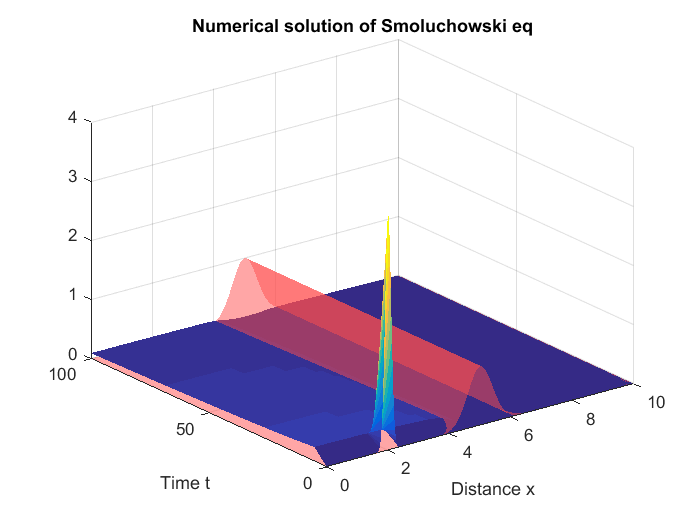
\includegraphics[width=0.9\linewidth]{./serf1}
\caption{Surface plot of the time x space grid with the potential barrier and the probability distribution}
\label{fig:surf}
\end{figure}
%
\begin{figure}
\centering
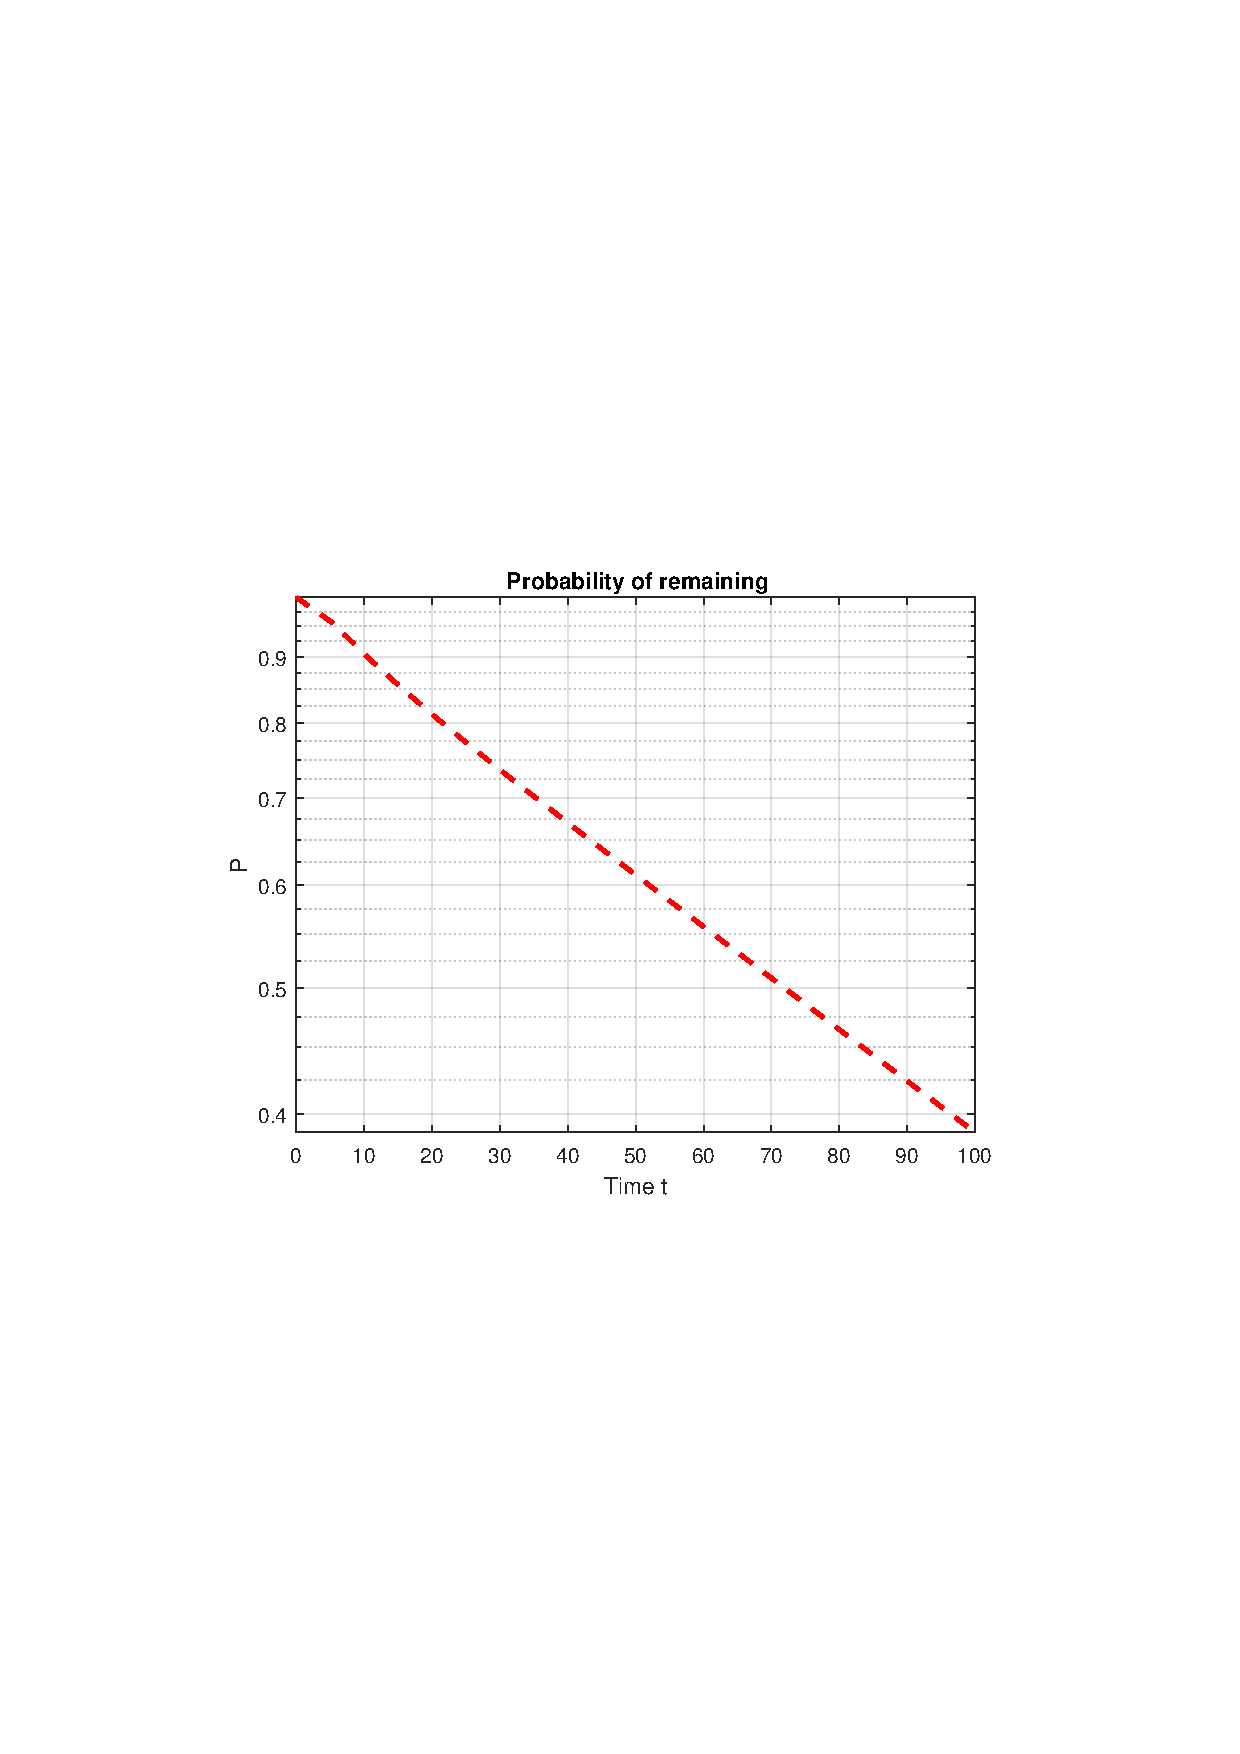
\includegraphics[width=1\linewidth]{./prob_remaining}
\caption{Probability of remaining confined to the left of the barrier as function of time: semilogy scale}
\label{fig:prob_remaining}
\end{figure}

\begin{figure}
\centering
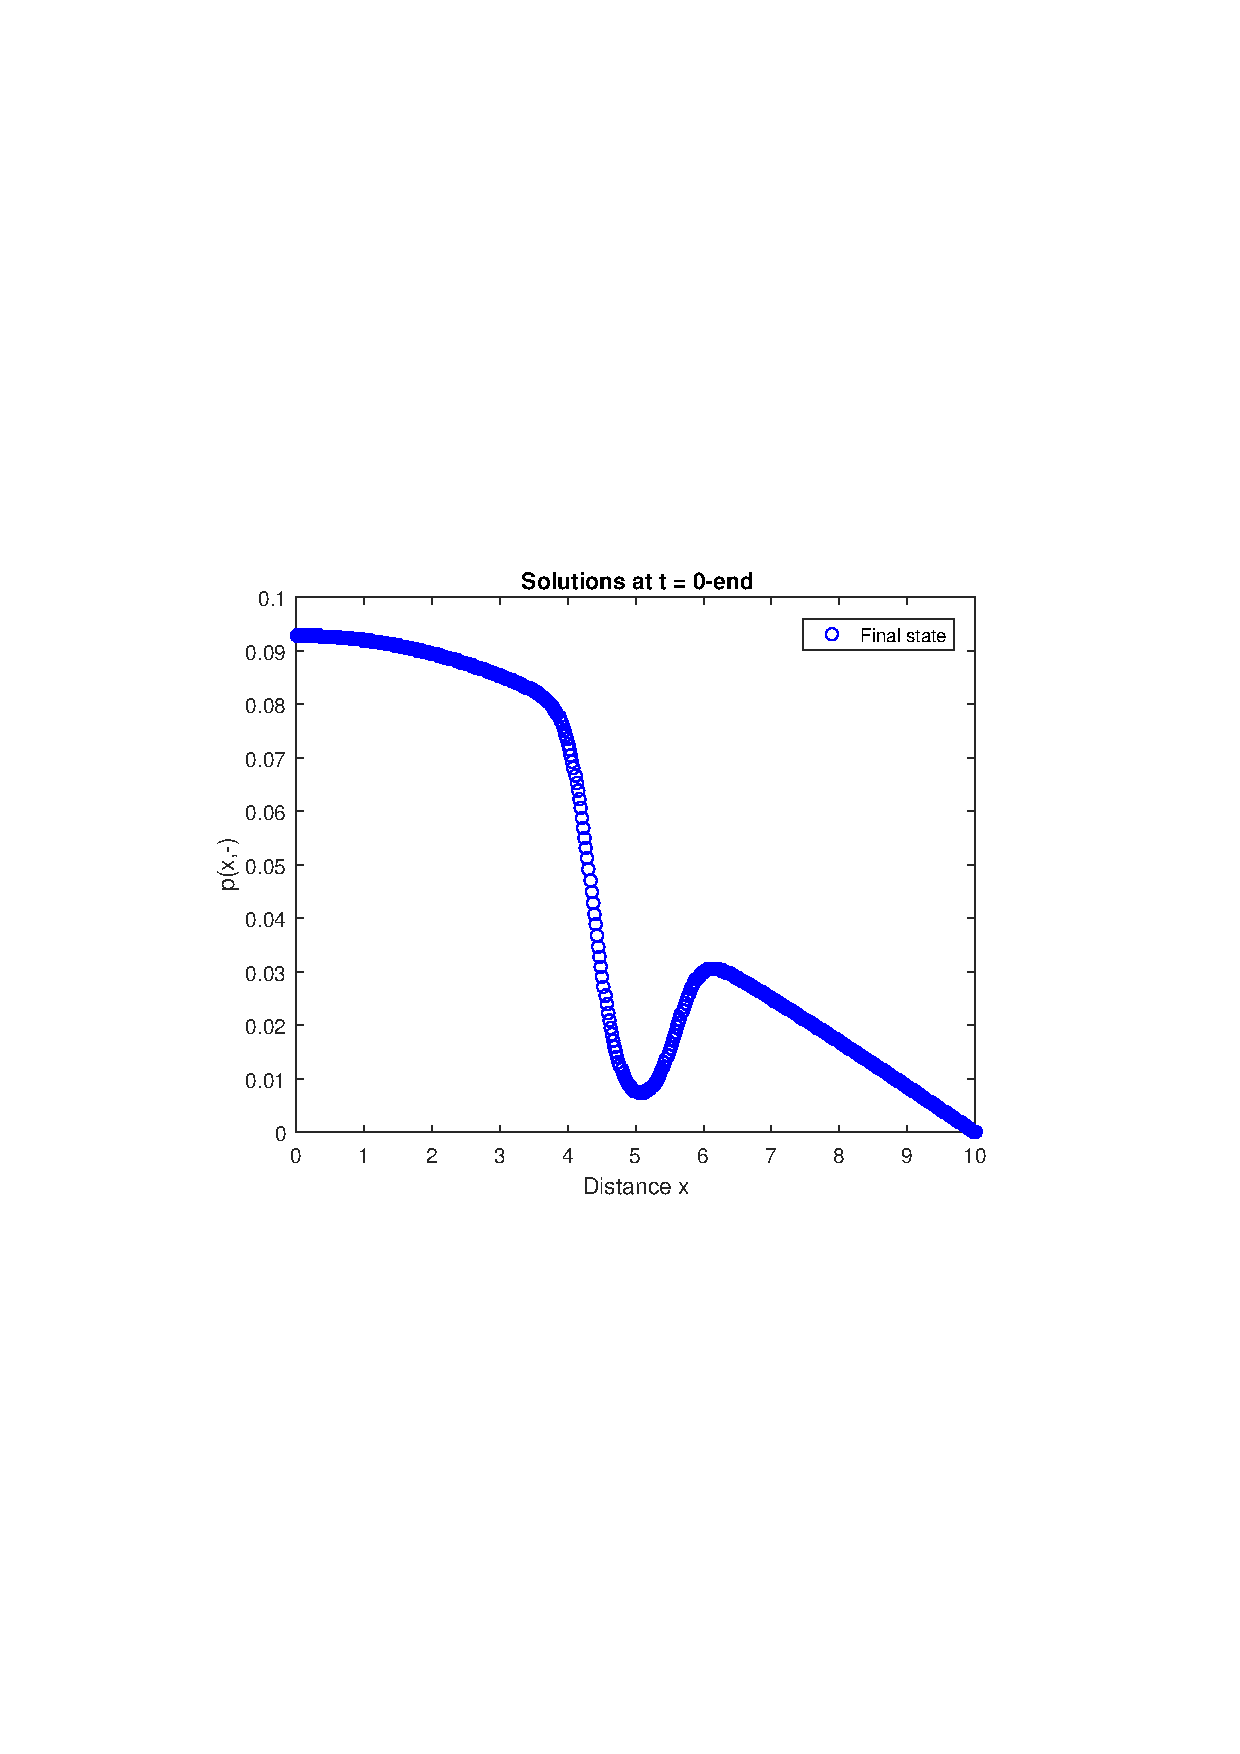
\includegraphics[width=1\linewidth]{./profile}
\caption{Profile of the probability distribution over the spatial domain for $t_{final} = 100$s.}
\label{fig:profile}
\end{figure}

\begin{figure}
\centering
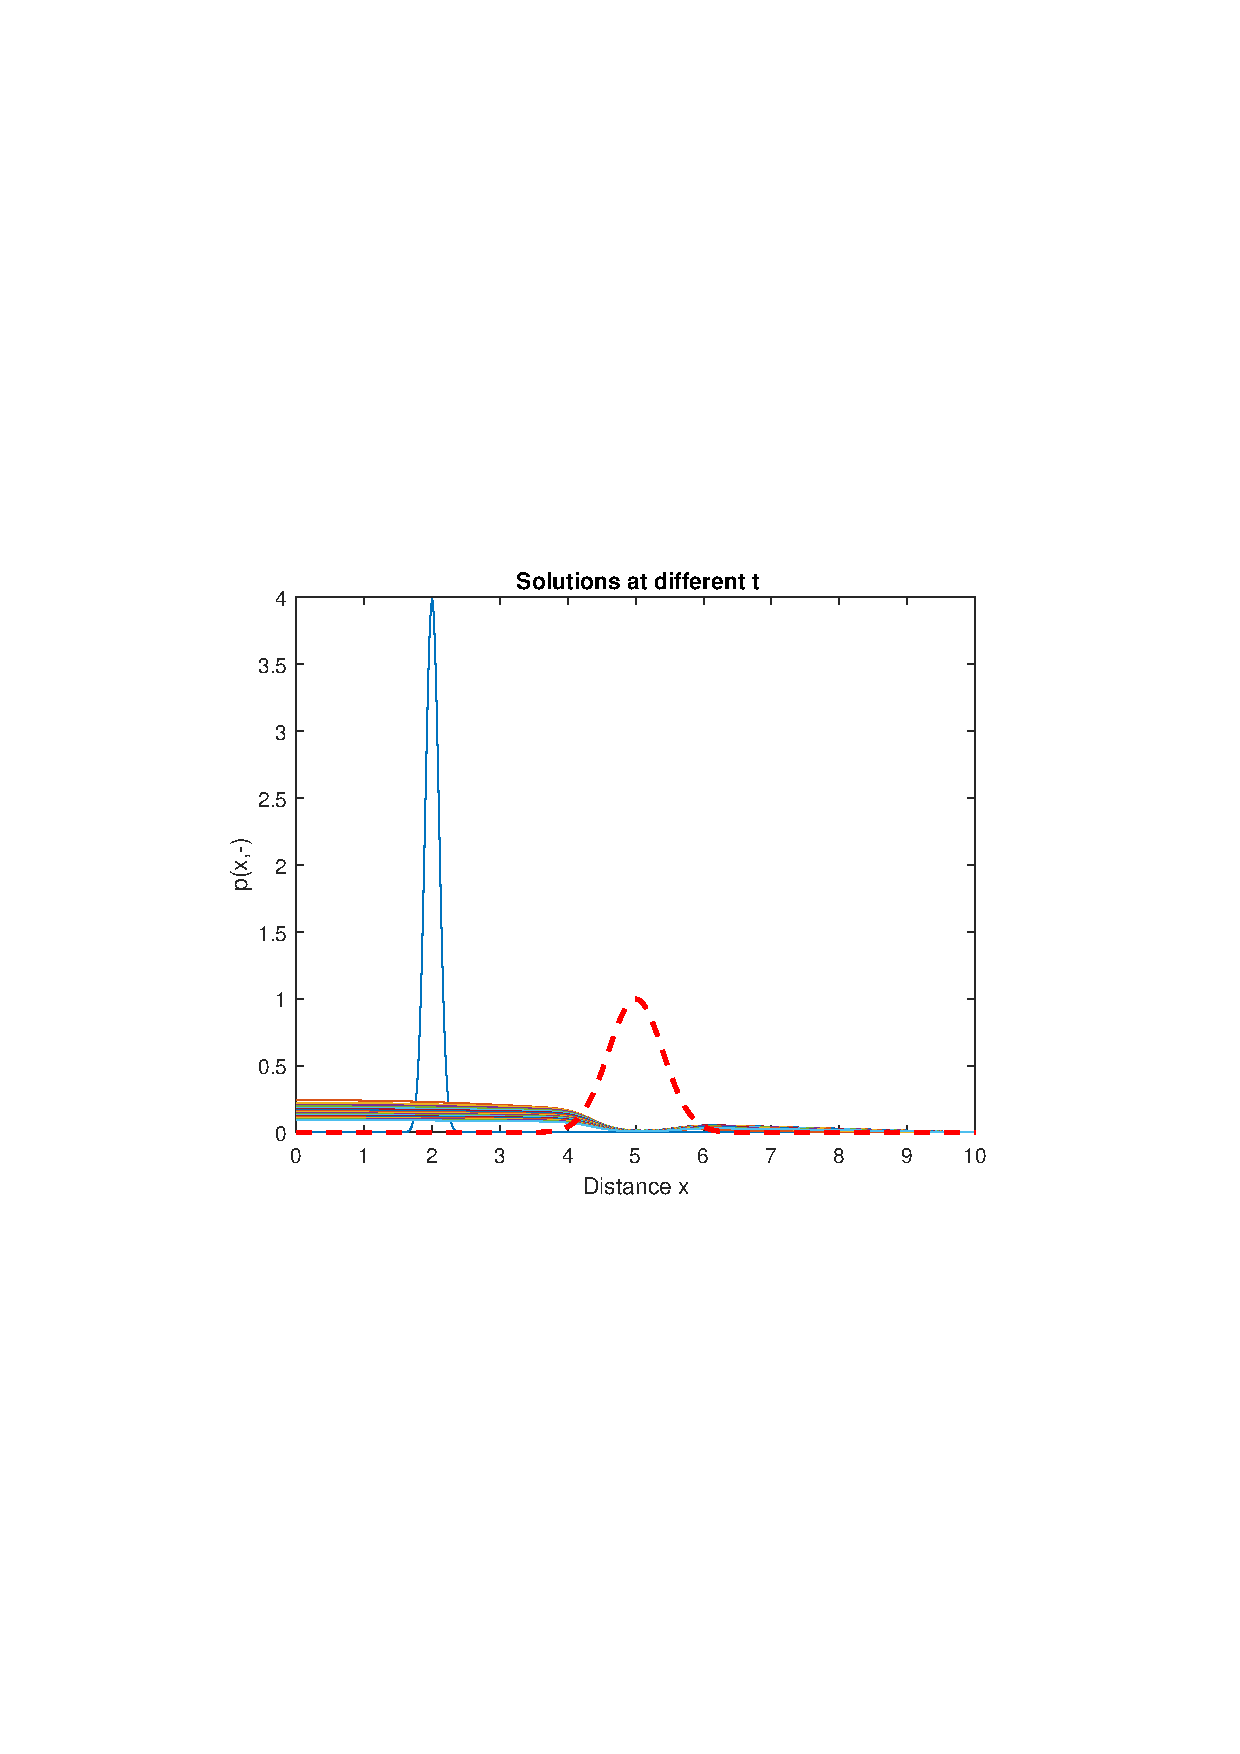
\includegraphics[width=1\linewidth]{./different_times}
\caption{Probability distribution for different t on the grid.}
\label{fig:different_times}
\end{figure}

\begin{figure}
\centering
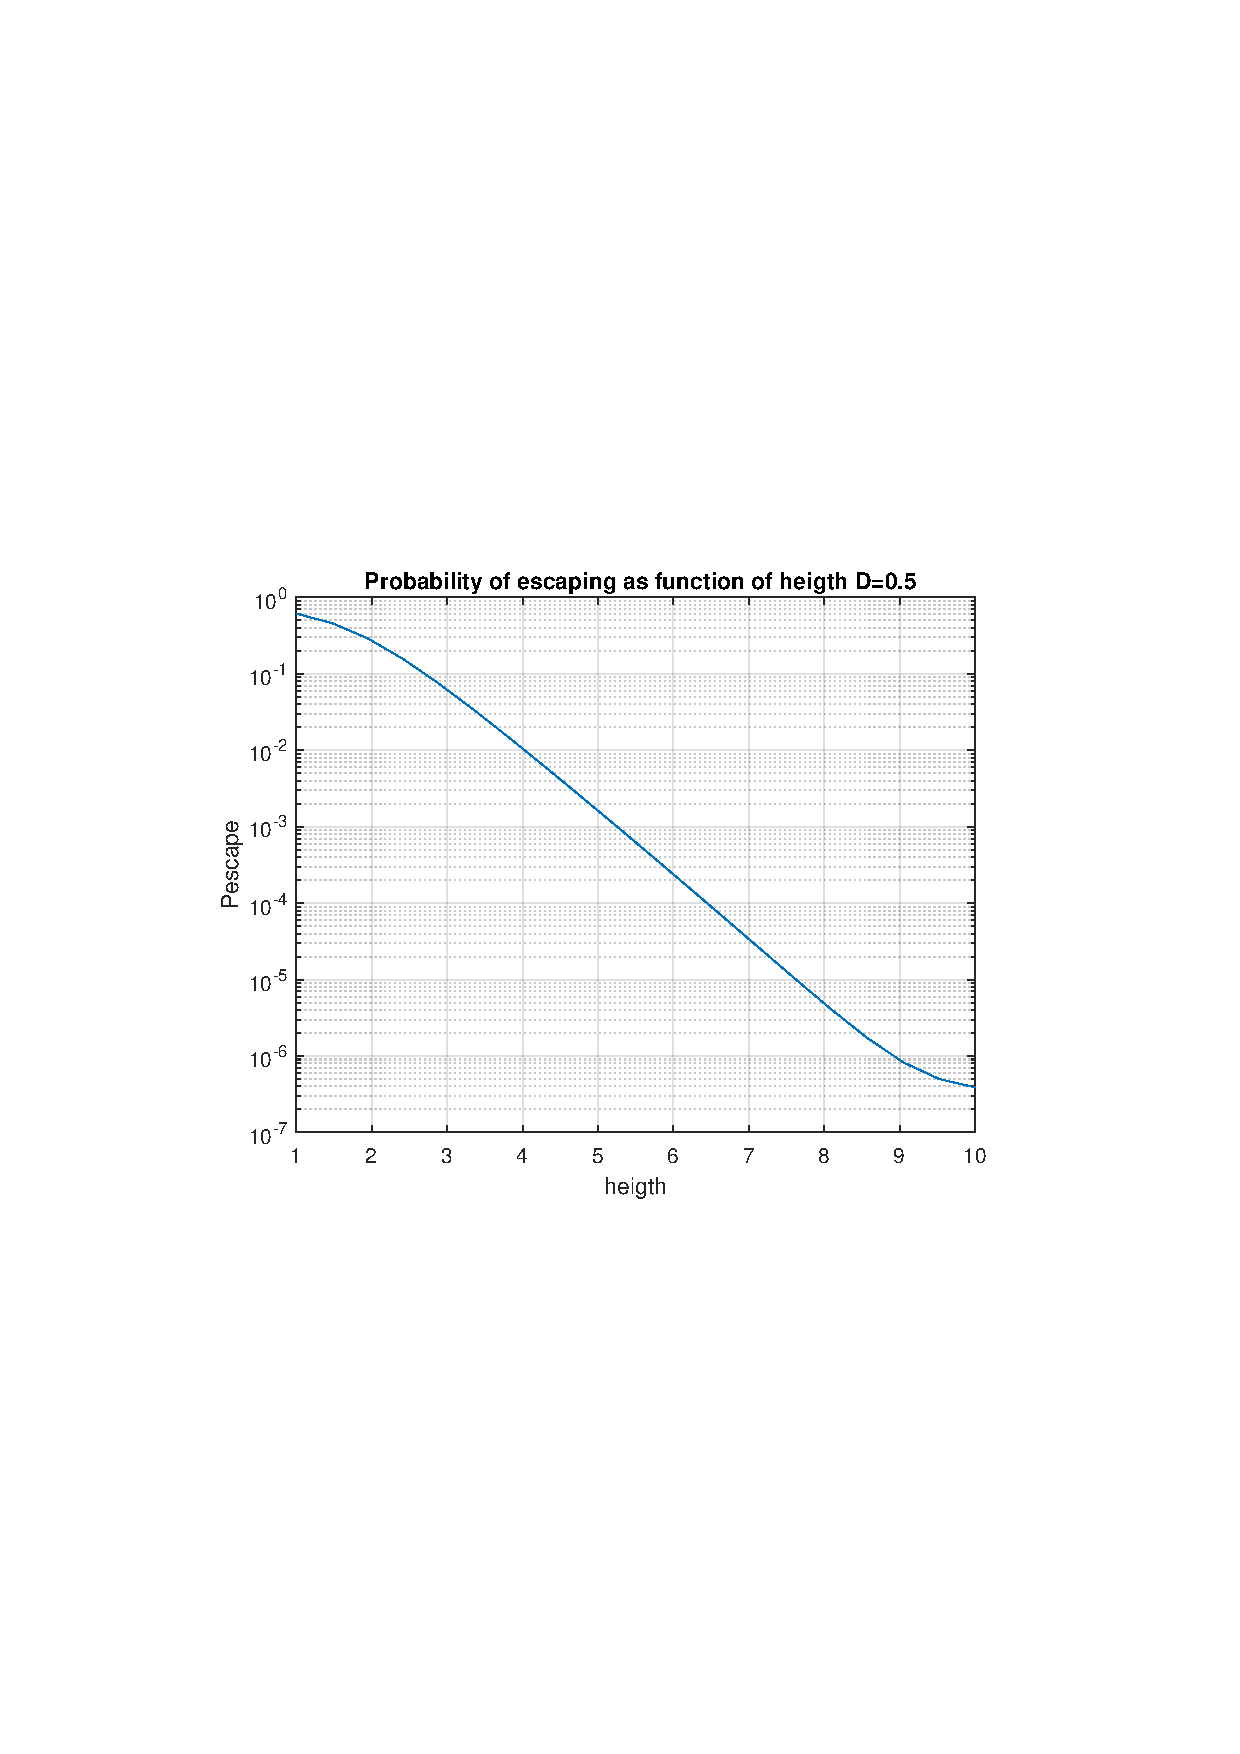
\includegraphics[width=1\linewidth]{./arrhenius05}
\caption{Semilogy plot of the escape probability as function of the height of the barrier: D = 0.5, t = 100s.}
\label{fig:arrhenius05}
\end{figure}

\begin{figure}
\centering
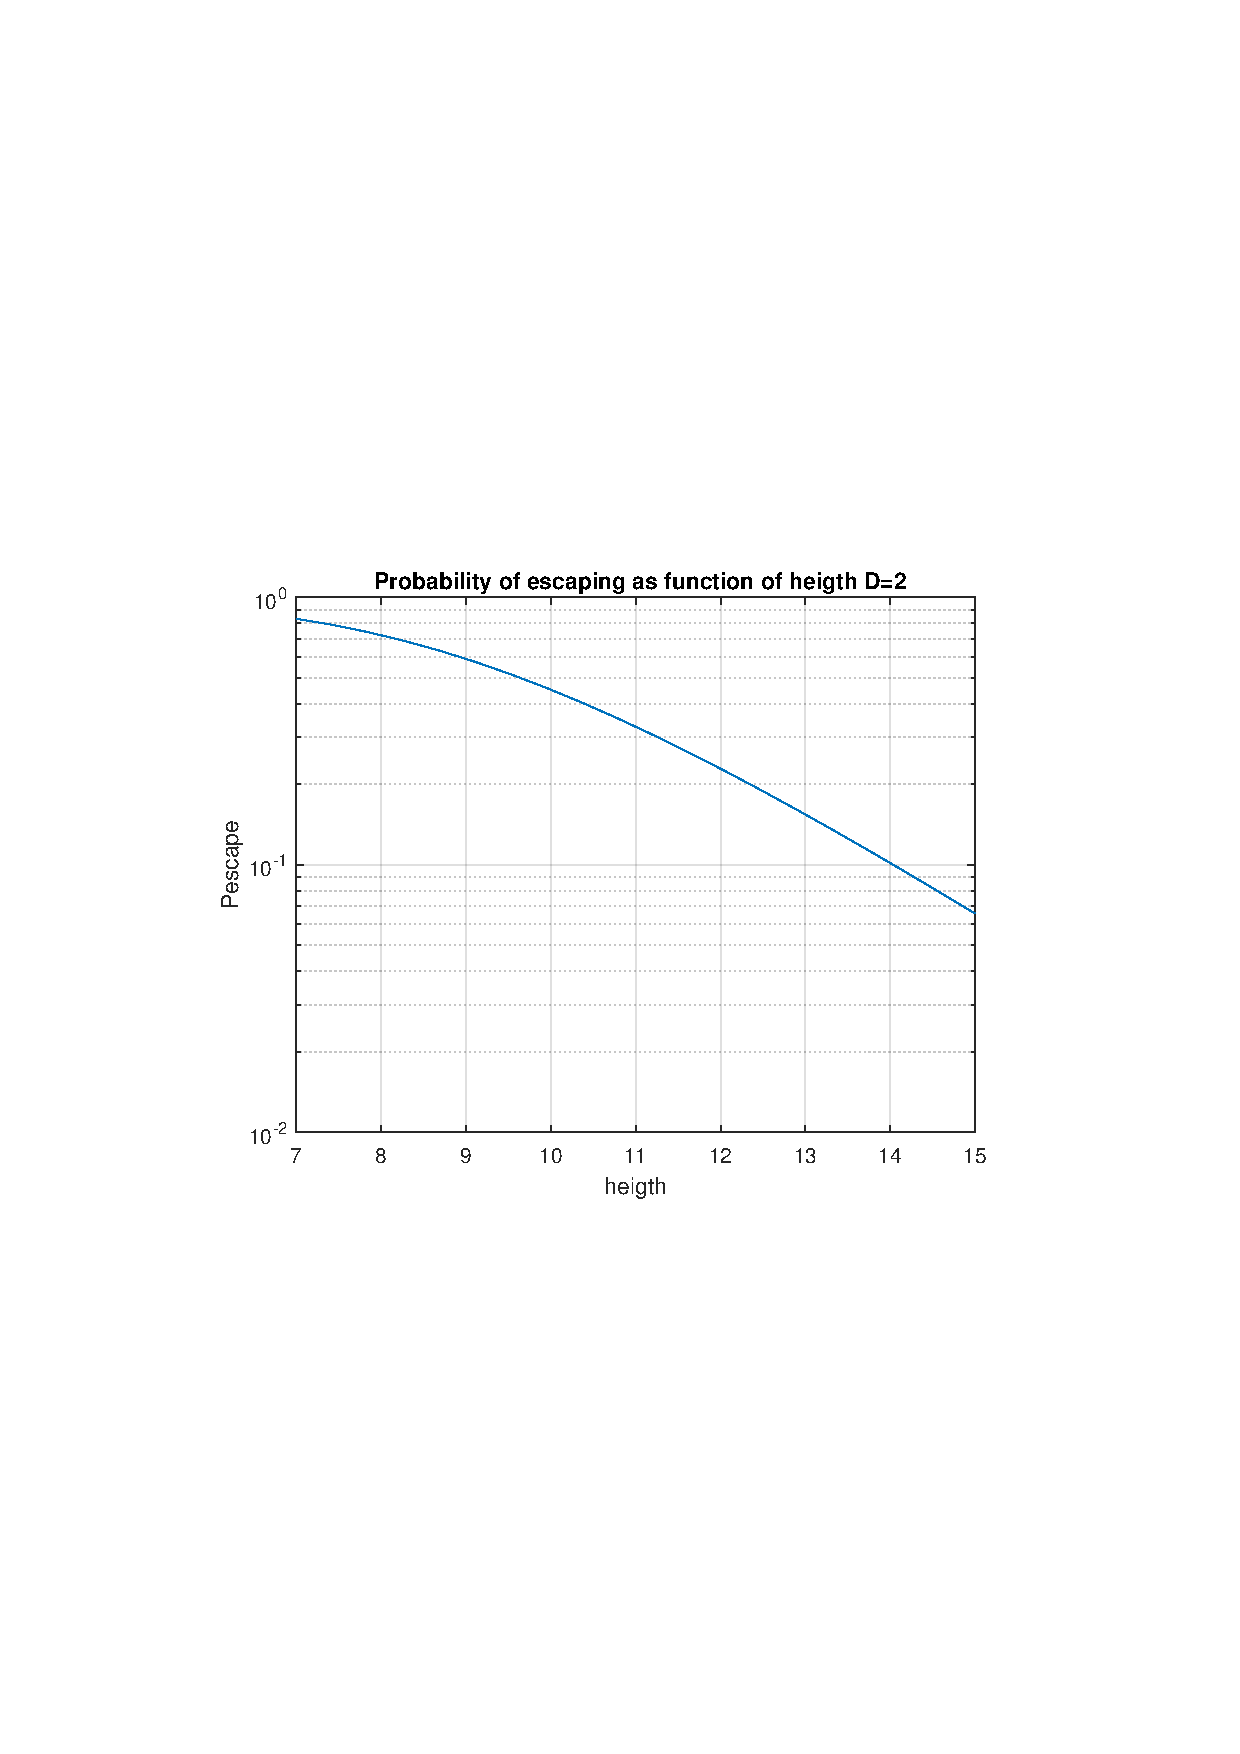
\includegraphics[width=1\linewidth]{./arrhenius2}
\caption{Semilogy plot of the escape probability as function of the height of the barrier: D = 2, t = 100s.}
\label{fig:arrhenius2}
\end{figure}

\end{document}